\chapter{Developing common representations in AI and humans}
\label{chap:common_representations}

In this Chapter we study how human representation and AI representation can be combined, and how brain data can be infused into neural networks.

\section[Using human brain activity to guide machine learning]{\textit{Using human brain activity to guide machine learning}\\ \mandatory{fong2017using}}

This study tries to \textbf{improve ML performance by guiding it with brain activity}, and explore whether such guidance makes the representations themselves more ``human-like". Notice that here the focus is not on performance but on \textbf{representational geometry}. The underlying idea is that, if the human brain is a natural reference point (for representation geometry) and performance, and ANNs are a good algorithm for learning structure, then we can attempt to leverage the ML algorithm with biological information.\\

They consider 7 brain areas (ROIs, \textit{regions of interest}, whose partitioning is defined a-priori). Different brain areas code for different information about the stimulus, but all of them are involved in \textbf{visual processing} (either low, middle, or high level). They use two types of models: CNN and HOG (\textit{histogram of oriented gradients}, an often-used algorithm for generating features that capture the local ``slopeness" of different parts of an image).

Their idea is to train a classifier on brain data to perform binary classification. To do so (to maximize the margin between the decision boundary and the data points), they use a loss derived from the \textbf{Hinge loss} \notet. They define the \textbf{``response strength" from brain fMRI activity data} as the \textbf{distance of an object from the decision boundary} for a given binary classification task.
This produces a per-stimulus activity weight (response strength) for each stimulus. As input to the classifier, each image is encoded as a vector of brain activity values sampled from a given brain area (one of the 7 mentioned before).
From the Hinge loss they define the \textbf{Activation weighted loss} (AWL) as:
\[
\phi (x, z) = max(0, (1-z) \cdot M(x,z)
\]
where $M(x,z) =\begin{cases}
         1+c_x, \text{if } z<1\\
        1 \text{ otherwise}
        \end{cases}$

and $c_x \geq 0$ is an activity weight derived from fMRI data corresponding to $x$ (it is the distance of the object from the classification boundary of the binary classifier trained on brain data).\\
While HL penalizes misclassified examples, \textbf{AWS penalizes misclassified examples on stimuli that are easy for humans to distinguish}.\\

They train a classifier on brain responses (fMRI), then use this prior knowledge to train a new model on non-annotated data. They basically use the learned weights as a starting point. The process consists in the following steps:
\begin{enumerate}
    \item \textbf{Derive per-stimulus ``activity weigths" from fMRI data}:
        \begin{itemize}
        \item collect \textit{per-stimulus} activity vectors: use fMRI to record bold response of subject;
        \item train a classifier on fMRI activity vectors: SVM classifier trained and tested;
        \item activity weights derived from distance boundary: use transformed classification scores.
    \end{itemize}
    \item \textbf{Train (calibrate) 2 image classifiers}:
    \begin{itemize}
        \item Conventional image classifier training: Radial Basis Function SVM classifier;
        \item Margins reweighted by activity data: SVM classifier with activity weighted loss function (note that not all training samples require fMRI weight).
    \end{itemize}
\end{enumerate}

They use images from 5 categories, and the classification problems are based on CNN or HOG features. Information from the higher-level cortical regions is combined in all possible combinations to produce feature sets.

\boxc{\notet Hinge loss}{
The true label is denoted as $t$ ($t=1$ or $t=-1$), while $y$ is the predicted activation for an object by the classifier. $t \cdot y$ is therefore the distance from the boundary. The Hinge loss wants to push this distance so that the margin from the boundary is above 1: 
\[
Loss(y) = max(0, 1-ty)
\]
if $ty <0$ (i.e., incorrect classification) $\Rightarrow 1-ty > 1$;\\
if $0< ty <1$ (correct classification but below the margin) $\Rightarrow 1-ty>0$;\\
if $ty>1$ (correct classification above the margin) $\Rightarrow  1-ty < 0$.\\
This means that the HL is proportional to the distance from the decision boundary, and it \textbf{does not care about magnitude of correct decisions above the margin}.\\

However, in \cite{fong2017using} they use a different formulation:
\[
\phi_h(z) = max(0,1-z)
\]
where $z = y \cdot f(x)$, $y \in N$ is the true label, and $f(x) \in \mathbb{R}$ is the predicted output; thus, $z$ denotes the correctness of a prediction. The HL function assigns a penalty to all misclassified data that is proportional to how erroneous the prediction is.
}

\subsection{Results}
They argue that brain activity compensates for poor feature representation (consider the large difference for HOAG in Figure \ref{fig:fong}).

\begin{figure}[!ht]
    \centering
    \captionsetup{width=.8\linewidth}
    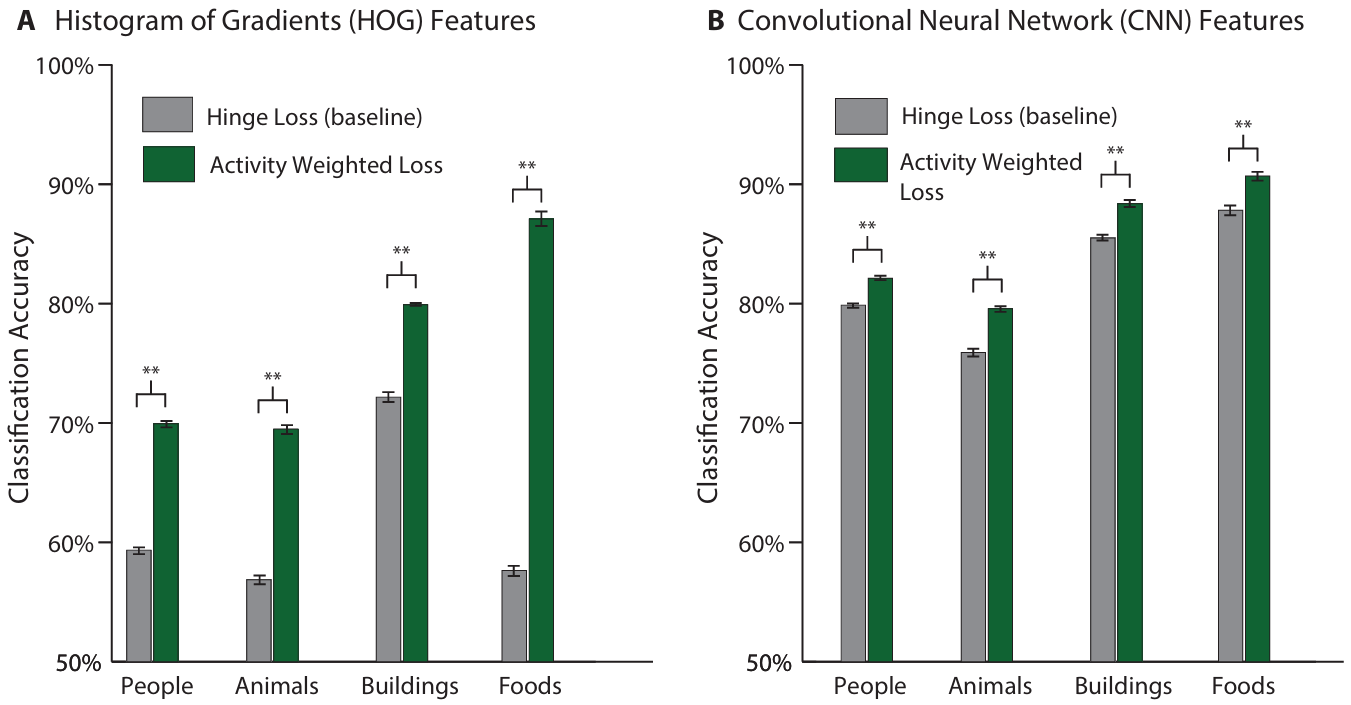
\includegraphics[width=0.6\linewidth]{images/fong.png}
    \caption{Side-by-side comparisons of the mean classification accuracy between models that were trained using either \textbf{(A)} HOG features or \textbf{(B)} CNN features and either a hinge loss (HL) or activity weighted loss (AWL) function.}
    \label{fig:fong}
\end{figure}

They also experiment using information from one brain area only for the loss, observing how this affects classification. Figure \ref{fig:fong_2} shows that certain areas produce significantly better accuracy for the specific categories they are selective for.\\

\begin{figure}[!ht]
    \centering
    \captionsetup{width=.8\linewidth}
    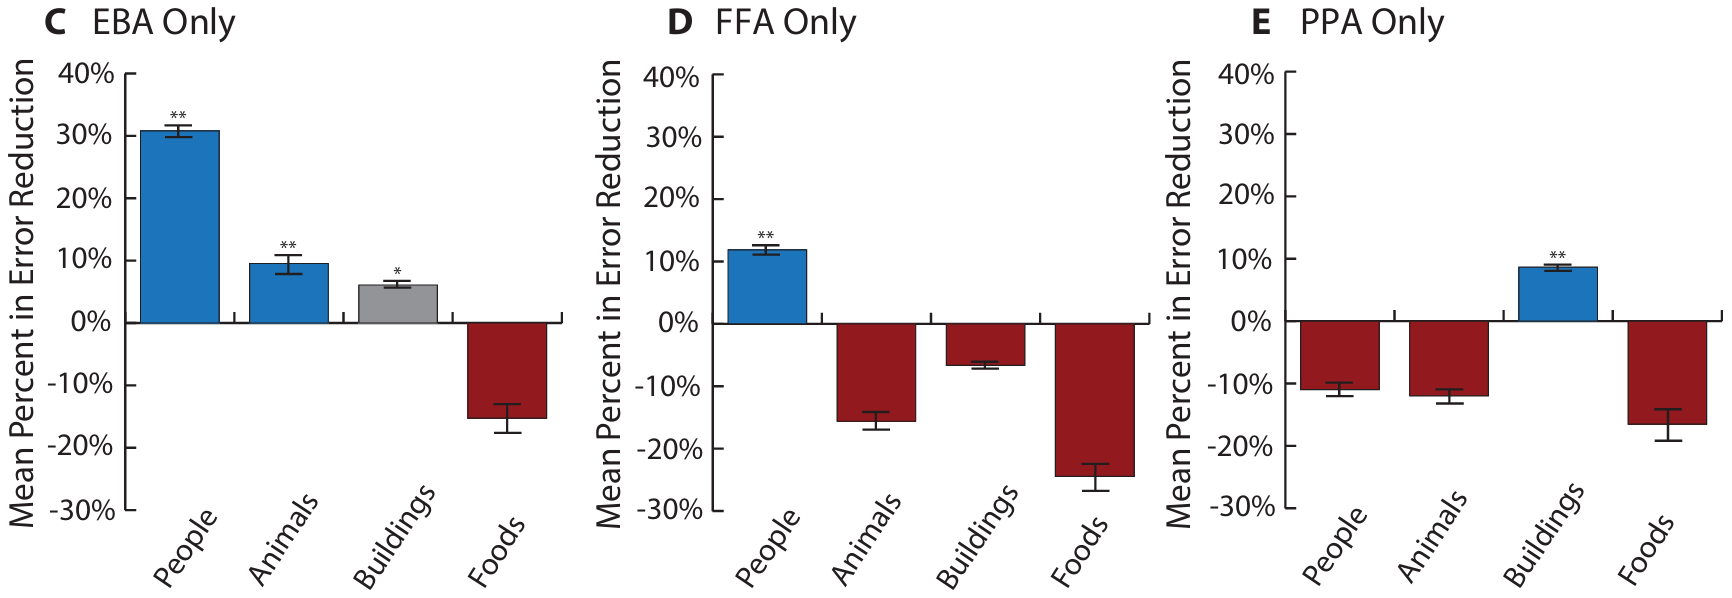
\includegraphics[width=0.6\linewidth]{images/fong_2.png}
    \caption{Mean error reductions gained by switching from HL to AWL loss when using conditioning classifies on brain activity from individual ROIs (i.e., EBA, FFA, or PPA).}
    \label{fig:fong_2}
\end{figure}

In conclusion, \textbf{information measured directly from brain can guide an ML algorithm to make better human-like decisions}.
One can harness measures of the internal representations employed by the brain to guide machine learning.
However, the authors ignore an important question: Are the better results obtained thanks to \textbf{brain} data, or is it just because it is \textbf{more} data? What if we improved the HOG classifier using AWL from CNN classifier (i.e., what if we compute the $C_x$ of the hinge loss from the CNN embeddings?).
The accuracy should be much higher, so we expect the difference when using Activity Weighted Loss to be less significant.
